\documentclass{article}
\usepackage{siunitx}
\usepackage{graphicx}
\usepackage{hyperref}
\title{AE2100 WP 1.1}
\author{Group C3}
\begin{document}
\maketitle
\subsection*{Task B}
% Define the mission elements with which the design process will
% interact (e.g.: mission operations, ground system, launch system,
% etc.).

The mission elements with which the design will have to interact are
the following.

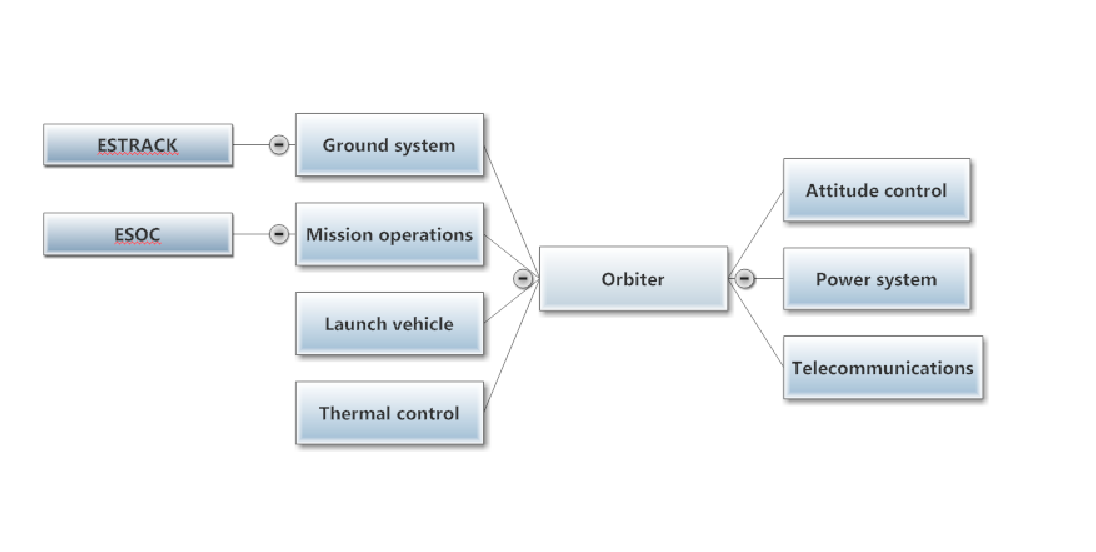
\includegraphics[scale=.65]{block-diagram-WP1-1B.eps}

\begin{itemize}
\item{Ground system.} The ground segment will use ESTRACK.
\item{Mission Operations Centre.} ESOC.
\item{Launch vehicle.}
\item{Thermal control.}
\item{Attitude control.}
\item{Power system.}
\item{Telecommunications.}
\end{itemize}

\subsection*{Task E}
\begin{itemize}
  \item{Payload mass.} 80 \si{kg}.
  \item{Payload dimensions.} 0.7m x 0.7m x 0.7m
  \item{Payload required power.} 50 W
  \item{Payload operational temperature range}
  \item{Orbit.} polar, 200 km above Europa surface
  \item{Mission duration.} At least 3 years in Europa orbit.
  \item{Launch date.} 2020.
  \item{Total mission cost.} Less than 500 million FY2000 USD.
\end{itemize}
\section*{WP 1.2}
\subsection*{Task A}
From \url{http://solarsystem.nasa.gov/planets/profile.cfm?Object=Jup_Europa&Display=Facts&System=Metric} and miscellaneous.
\begin{itemize}
\item{Orbit Size Around Jupiter (semi-major axis):}  671,100 km
\item{Periapsis (closest):}  664,792 km
\item{Apoapsis (farthest):}  677,408 km
\item{Sidereal Orbit Period (Length of Year):} 3.551181041 Earth days
\item{Orbit Circumference:}  4,216,552.51 km
\item{Average Orbit Velocity:}  49,476.1 km/h
\item{Orbit Eccentricity:} 0.0094
\item{Orbit Inclination:} 0.466 degree
\item{Mean Radius:}  1,560.8 km
\item{Equatorial Circumference:}  9806.8 km
\item{Volume:}  15,926,867,918 \si{km^3}
\item{Mass:}  47,998,438,387,492,700,000,000 kg
\item{Planet density:}  3.013 \si{g/cm^3}
\item{Surface Area:}  30,612,893.23 \si{km^2}
\item{Surface Gravity:}  1.315 \si{m/s^2}
\item{Escape Velocity:}  7,293 km/h. Scientific Notation: 2026 m/s
\item{Sidereal Rotation Period (Length of Day):} 3.551 Earth days
\item{Atmospheric Constituents:} Oxygen
\item{Temperature:} 102K
\item{Albedo:} 0.67
\item{Solar intensity:} 49.8 \si{W/m^2}
\end{itemize}aa
\end{document}
